\subsection{Estrutura do Trabalho} \label{subsec:estrutura}


O trabalho está estruturado em diferentes capítulos, cada um abordando aspectos específicos da pesquisa. 
O Capítulo~\ref{sec:int}, Introdução, apresenta a introdução do trabalho, fornecendo uma contextualização do estudo, destacando a motivação e os objetivos a serem alcançados. Também são apresentados o problema em questão, a metodologia utilizada, a justificativa da pesquisa, as contribuições esperadas e a organização do trabalho.

O Capítulo~\ref{sec:refteo}, Revisão Teórica, oferece uma visão geral das principais pesquisas e estudos relacionados às questões abordadas na pesquisa. Aquele capítulo proporciona uma base teórica sólida para fundamentar a análise e interpretação dos resultados.

No Capítulo~\ref{sec:base}, são apresentados os modelos que serão utilizados para trabalhar com os dados coletados. Aquela seção detalha os modelos escolhidos, destacando suas características e fundamentos teóricos. Além disso, é realizado o detalhamento do estudo de caso utilizado na dissertação.


O Capítulo~\ref{sec:result}, Resultados, apresenta os resultados obtidos ao longo da pesquisa. Naquela seção, são realizadas análises e interpretações dos resultados, fornecendo entendimento relevantes para o problema em estudo. Os resultados do estudo de caso são detalhados, evidenciando as principais descobertas e conclusões obtidas.

Por fim, o Capítulo~\ref{sec:conclusoes}, Conclusões, traz as considerações finais da pesquisa. Também são apresentadas propostas para pesquisas futuras, visando expandir e aprofundar o conhecimento na área.

Este documento está estruturado em~\ref{sec:conclusoes} capítulos, divididos como mostrado na Figura \ref{fig:estrutura}.
 
 \begin{figure}[H]
 	\centering
 	\caption{Estrutura da dissertação}
 	\label{fig:estrutura}
 	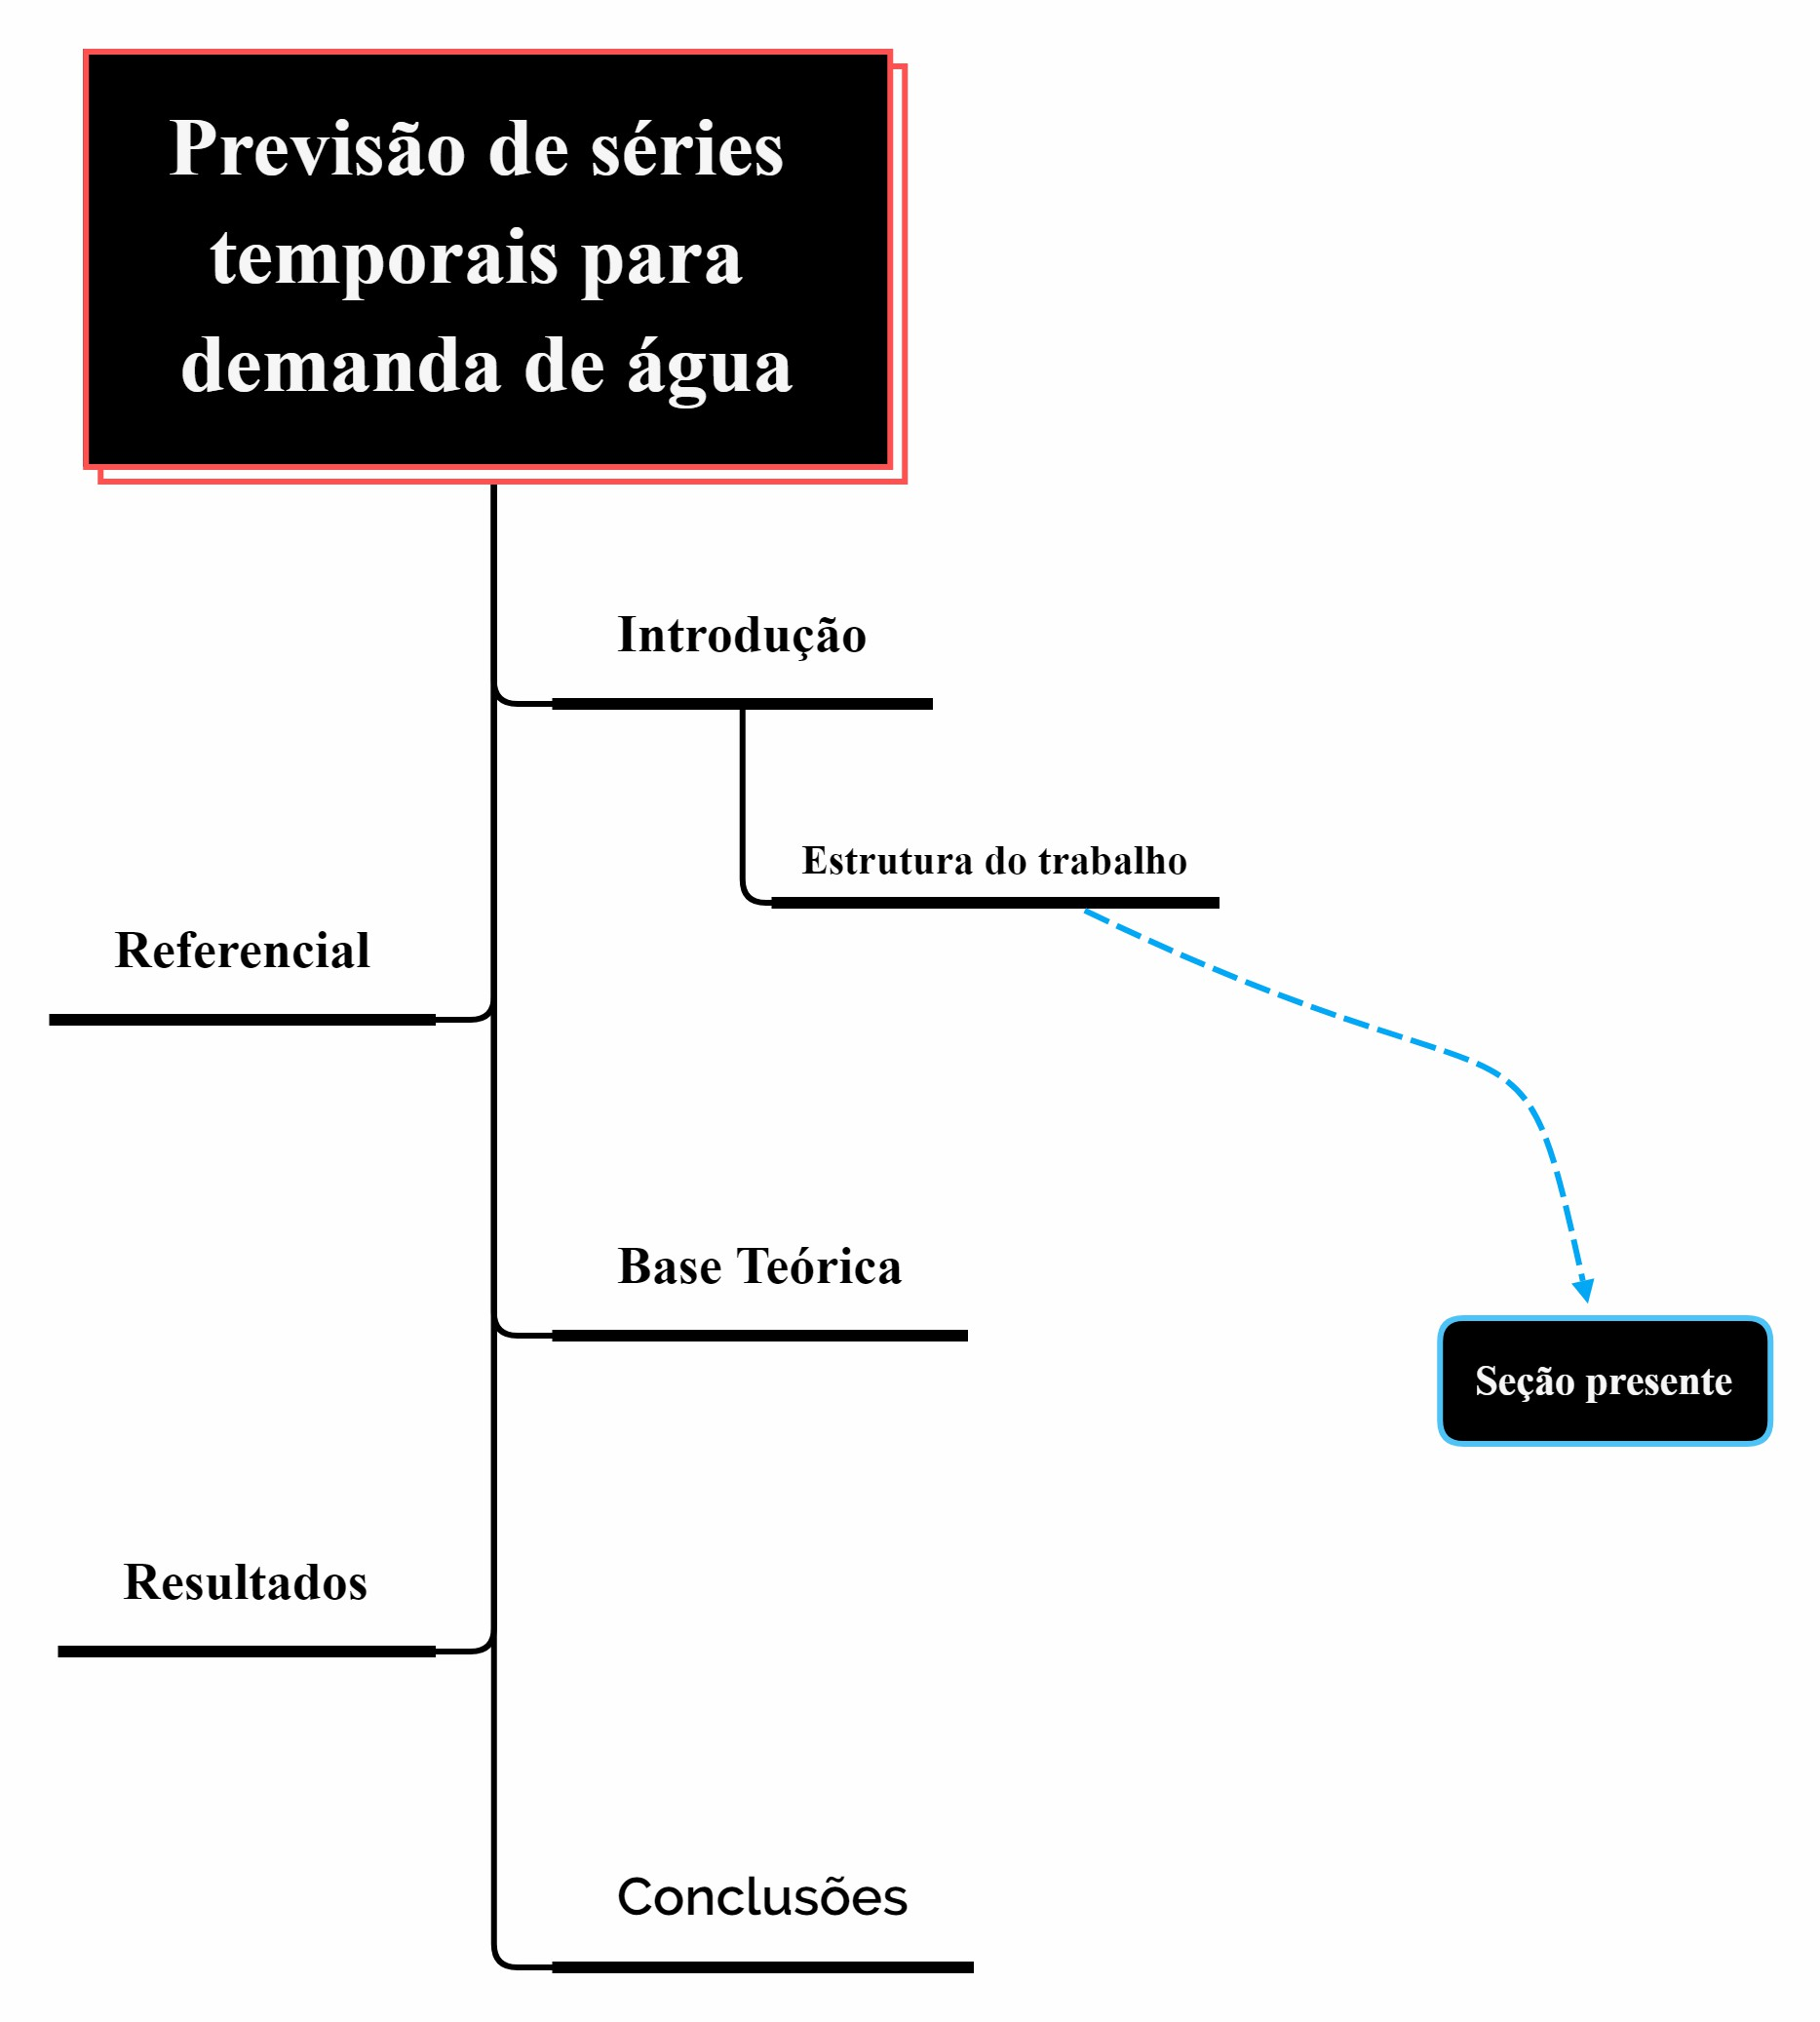
\includegraphics[width=\linewidth]{Introducao/Figuras/Estrutura}
 	
 	\fonte{Elaboração própria} 
 \end{figure}



